\documentclass[11pt,a4paper]{article}

% ==============================================================================
% PACKAGES FOR SINGLE-COLUMN 10-PAGE RESEARCH PAPER LAYOUT
% ==============================================================================
\usepackage[utf8]{inputenc}
\usepackage[T1]{fontenc}
\usepackage{geometry}
\geometry{margin=0.95in}
\usepackage{times}
\usepackage{amsmath,amssymb}
\usepackage{graphicx}
\usepackage{booktabs}
\usepackage{array}
\usepackage{multirow}
\usepackage{algorithm}
\usepackage{algpseudocode}
\usepackage{hyperref}
\usepackage{xcolor}
\usepackage{caption}
\usepackage{subcaption}
\usepackage{enumitem}
\usepackage{float}

\hypersetup{
    colorlinks=true,
    linkcolor=blue!70!black,
    citecolor=blue!70!black,
    urlcolor=blue!70!black
}

\setlength{\parskip}{0.45em}
\setlength{\parindent}{0em}

% ==============================================================================
% PAGE 1: FRONT MATTER & INTRODUCTION
% ==============================================================================
\title{\textbf{Comparative Evaluation of Classical and Deep Learning OCR Engines Across Multilingual and Degraded Document Conditions}}

\author{
    \textbf{Ritik Kumar} \\
    School of Computer Science Engineering \& Technology \\
    \texttt{https://github.com/RitikKumarS24/OCR-Comparison-Project}
}

\date{}

\begin{document}
\maketitle

\begin{abstract}
Optical Character Recognition (OCR) systems are foundational to automated document digitization, archival indexing, and enterprise workflow automation. However, real-world scanned and mobile-captured documents routinely suffer from sensor noise, motion blur, geometric skew, and low spatial resolution—degradations that severely degrade recognition fidelity. Furthermore, multilingual digitization in South Asia demands simultaneous accuracy across both Latin (English) and Devanagari (Hindi) scripts, where continuous upper headlines (\textit{shirorekha}), stacked consonant conjuncts, and sub-baseline vowel modifiers (\textit{matras}) violate the character-segmentation assumptions of traditional OCR pipelines. In this work, we present an end-to-end, reproducible benchmarking framework evaluating five representative OCR architectures—spanning classical connected-component BiLSTM models (\textbf{Tesseract v5}), deep CNN-RNN scene and document pipelines (\textbf{EasyOCR}, \textbf{PaddleOCR v3.7}, \textbf{docTR v1.1}), and Vision-Language Encoder-Decoder Transformers (\textbf{SuryaOCR v0.17})—across 100 bilingual document images under five controlled degradation conditions (\texttt{original}, \texttt{noisy}, \texttt{blurry}, \texttt{rotated}, and \texttt{low\_resolution}) and two processing pipelines (\texttt{raw} versus adaptive \texttt{OpenCV} restoration), totaling 1,000 quantitative evaluations. Using canonical Unicode NFC normalization alongside Character Error Rate (CER), Word Error Rate (WER), and inference latency, our experiments reveal critical architectural trade-offs: \textbf{SuryaOCR} and \textbf{PaddleOCR} tie at \textbf{99.79\%} English character accuracy, while \textbf{SuryaOCR} leads decisively on Hindi at \textbf{97.71\%} (\textbf{0.0229} CER), outperforming classical and CRNN peers by over 9 percentage points. Conversely, adaptive OpenCV preprocessing reduces Tesseract's English CER by \textbf{81.9\%} (achieving \textbf{99.22\%} accuracy in \textbf{0.268\,s/image}), establishing a clear Pareto frontier between real-time throughput and multilingual transformer accuracy.
\end{abstract}

\textbf{Keywords:} Optical Character Recognition (OCR), Multilingual Document Analysis, Devanagari Script, Vision Transformers, Image Restoration, OpenCV Preprocessing, Character Error Rate (CER), Benchmarking.

\section{Introduction}
Large-scale digitization of administrative records, legal archives, academic literature, and financial receipts relies heavily on Optical Character Recognition (OCR) to convert unstructured raster imagery into searchable, machine-readable text. Despite rapid advances in deep learning, deploying OCR engines in heterogeneous production environments remains challenging due to two compounding factors: \textit{physical image degradation} and \textit{orthographic script diversity}. Document images acquired via flatbed scanners, mobile cameras, or legacy microfilm frequently exhibit additive Gaussian or salt-and-pepper sensor noise, defocus and motion blur, rotational skew, and severe downsampling. Even minor pixel-level distortions can fracture stroke connectivity, causing brittle character-level classifiers to hallucinate or drop characters.

Equally critical is the linguistic gap between Latin-script benchmarks and complex Indic scripts such as Devanagari (used for Hindi, Marathi, and Sanskrit). Unlike English, where characters are separated by explicit inter-glyph whitespace, Devanagari words are bound together horizontally by a continuous top header line known as the \textit{shirorekha}, while vowel signs (\textit{matras}) and diacritics (\textit{nukta}, \textit{anusvara}) attach above, below, or around base consonants. Traditional connected-component segmentation algorithms struggle to isolate individual glyphs beneath a shared \textit{shirorekha}, whereas modern sequence-to-sequence Vision Transformers process full text lines holistically without explicit character segmentation.

Existing OCR comparisons typically evaluate engines solely on clean English datasets or report aggregate accuracy without isolating the impact of image preprocessing or script-specific Unicode normalization. To bridge this gap, this paper makes the following core contributions:
\begin{itemize}[leftmargin=1.4em]
    \item \textbf{Controlled Bilingual Degradation Benchmark:} We construct a reproducible 100-image bilingual evaluation corpus balanced equally between English and Hindi across five controlled visual conditions (\texttt{original}, \texttt{noisy}, \texttt{blurry}, \texttt{rotated}, and \texttt{low\_resolution}) with exact UTF-8 ground truth.
    \item \textbf{Adaptive Condition-Aware OpenCV Restoration Pipeline:} We design and evaluate a multi-branch OpenCV preprocessing module incorporating projection-profile deskewing, CLAHE contrast equalization, Otsu adaptive binarization, and $2\times$ bicubic super-resolution upscaling, quantifying its exact impact across all 1,000 benchmark runs.
    \item \textbf{Canonical Unicode NFC Evaluation & Pareto Analysis:} We enforce canonical Unicode NFC normalization to eliminate false CER/WER penalties on composite Devanagari code points and establish empirical speed-versus-accuracy Pareto frontiers guiding real-world system deployment.
\end{itemize}

\newpage
% ==============================================================================
% PAGE 2: RELATED WORK & BACKGROUND
% ==============================================================================
\section{Related Work}
Research in Optical Character Recognition has evolved across three distinct architectural paradigms: classical statistical and recurrent sequence models, modular deep convolutional-recurrent detectors and recognizers, and end-to-end Vision-Language Transformers.

\subsection{Classical Connected-Component and BiLSTM OCR}
Early OCR systems relied on explicit image binarization, connected-component analysis, line/word segmentation, and handcrafted topological features classified via Hidden Markov Models or Support Vector Machines. Smith~\cite{smith2007overview} introduced the modern open-source Tesseract architecture, which originally employed polygonal approximation and adaptive character classifiers before transitioning in Tesseract v4/v5 to a line-level Bidirectional Long Short-Term Memory (BiLSTM) network trained with Connectionist Temporal Classification (CTC) loss~\cite{graves2006connectionist,breuel2013high}. While BiLSTM-CTC eliminates the need for manual character-level bounding boxes during training, classical line-finding front-ends remain highly sensitive to page skew, uneven illumination, and salt-and-pepper noise, often requiring external morphological cleanup and binarization~\cite{otsu1979threshold,sauvola2000adaptive}.

\subsection{Deep CNN-RNN Modular Scene and Document Pipelines}
To handle arbitrary orientations, complex backgrounds, and multi-font documents, modern deep OCR frameworks decouple text localization from sequence transcription. For text detection, Baek et al.~\cite{baek2019character} proposed CRAFT (Character Region Awareness for Text Detection), predicting character-level affinity scores to group curved or spaced glyphs, while Liao et al.~\cite{liao2020real} introduced Differentiable Binarization (DBNet), integrating adaptive thresholding directly into a Feature Pyramid Network for real-time segmentation. Mindee's docTR~\cite{doctr2021} pairs fast reparameterized detection backbones (FAST~\cite{li2023fast}) with Convolutional Recurrent Neural Networks (CRNN~\cite{shi2016end}) using VGG-16 feature extractors. Similarly, Baidu's PaddleOCR series (PP-OCRv3 through PP-OCRv5)~\cite{du2020pp,li2022pp} combines lightweight DBNet detectors with Single Visual Model for Text Recognition (SVTR)~\cite{du2022svtr}, achieving strong industrial throughput across Latin and CJK scripts. However, CRNN-based recognizers constrained by fixed-height feature pooling frequently compress vertically stacked Devanagari \textit{matras}, leading to substitution errors in Hindi text.

\subsection{Vision-Language Transformers and Multilingual Devanagari OCR}
Inspired by the success of Vision Transformers (ViT)~\cite{dosovitskiy2020image} in image understanding, transformer-based OCR architectures replace recurrent CTC decoders with self-attention encoder-decoders capable of modeling long-range spatial and linguistic context. Li et al.~\cite{li2023trocr} demonstrated with TrOCR that pre-trained image and text transformers substantially outperform CRNN baselines on printed and handwritten benchmarks. Building on patch-based vision encoders and multi-resolution layout analysis, Paruchuri~\cite{paruchuri2024surya} developed SuryaOCR, an end-to-end multilingual document OCR and layout model supporting over 90 languages—including Devanagari—without brittle connected-component heuristics.

In the context of Indic document analysis, prior studies have documented the unique challenges of Devanagari recognition, including \textit{shirorekha} fragmentation, conjunct consonants (\textit{sanyuktakshars}), and Unicode canonical equivalence issues~\cite{pal2004indian,jawahar2003bilingual,dwivedi2020indic}. Yet existing literature lacks a unified, head-to-head empirical benchmark that systematically contrasts classical BiLSTM, modular CNN-RNN, and modern Vision Transformer engines across identical degraded English and Hindi documents under both raw and OpenCV-restored pipelines. Our work directly addresses this gap.

\newpage
% ==============================================================================
% PAGES 3-4: PROPOSED METHODOLOGY & EVALUATION PIPELINE
% ==============================================================================
\section{Proposed Methodology and Evaluation Architecture}

\subsection{System Overview and Benchmarking Pipeline}
To ensure strict experimental fairness across heterogeneous model architectures, we designed a modular four-stage evaluation framework (Figure~\ref{fig:pipeline}): (1) \textit{Synthetic Bilingual Dataset & Degradation Synthesis}, (2) \textit{Condition-Adaptive OpenCV Image Restoration}, (3) \textit{Unified OCR Inference Engine Wrappers}, and (4) \textit{Unicode-Normalized Error & Pareto Profiling}.

\begin{figure}[H]
    \centering
    \fbox{\parbox{0.94\textwidth}{
        \centering
        \vspace{0.4em}
        \textbf{[Bilingual Ground Truth Corpus: 10 English + 10 Hindi Passages]} \\
        $\downarrow$ \\
        \textbf{Stage 1: Controlled Degradation Generator} (\texttt{original}, \texttt{noisy}, \texttt{blurry}, \texttt{rotated}, \texttt{low\_res} $\rightarrow$ 100 Images) \\
        $\downarrow$ \hspace{6.5em} $\searrow$ \\
        \textbf{Branch A: Raw Pipeline} \hspace{3.2em} \textbf{Branch B: Adaptive OpenCV Restoration} \\
        \textit{(Direct RGB Input)} \hspace{4.8em} \textit{(Deskew + CLAHE / Otsu Denoise / $2\times$ Bicubic Upscale)} \\
        $\downarrow$ \hspace{6.5em} $\swarrow$ \\
        \textbf{Stage 3: 5 Unified OCR Engine Wrappers} (Tesseract, EasyOCR, PaddleOCR, docTR, SuryaOCR) \\
        $\downarrow$ \\
        \textbf{Stage 4: Canonical Unicode NFC Normalization \& Metrics} (CER, WER, Latency, Peak RAM $\Delta$)
        \vspace{0.4em}
    }}
    \caption{End-to-end dual-pipeline comparative OCR evaluation architecture executing $100 \times 2 \times 5 = 1{,}000$ controlled benchmark runs.}
    \label{fig:pipeline}
\end{figure}

Each of the 100 test images is evaluated twice per engine—once in its raw degraded form and once after adaptive OpenCV restoration—yielding $100 \times 2 \times 5 = 1{,}000$ paired observations. Every engine wrapper exposes a standardized interface returning transcribed text, wall-clock execution latency (measured after model initialization and CUDA warm-up), and process resident set size (RSS) memory delta.

\subsection{Adaptive OpenCV Restoration Module and Benchmark Pseudocode}
A single static preprocessing chain can harm certain degradations (for instance, aggressive global thresholding destroys anti-aliased strokes in low-resolution scans). Consequently, our \texttt{ImagePreprocessor} routes images through three specialized OpenCV restoration modes based on degradation characteristics:
\begin{itemize}[leftmargin=1.4em]
    \item \textbf{Standard Restoration Mode (\texttt{original}, \texttt{rotated}, \texttt{blurry}):} Converts input RGB imagery to single-channel grayscale, estimates skew angle $\theta$ via minimum-area bounding rectangles on foreground text contours, applies an affine rotation matrix $M(\theta)$ with white border replication to restore horizontal baseline alignment, enhances local stroke contrast via Contrast Limited Adaptive Histogram Equalization (CLAHE, clip limit $= 2.0$, tile grid $= 8 \times 8$), and sharpens blurred edges using unsharp masking ($I_{\text{sharp}} = 1.5\,I - 0.5\,G_{\sigma}(I)$).
    \item \textbf{Binary Denoising Mode (\texttt{noisy}):} Applies a $3 \times 3$ median filter to suppress impulse salt-and-pepper speckles followed by Gaussian smoothing ($\sigma = 0.8$), performs global Otsu thresholding~\cite{otsu1979threshold} to separate foreground ink from background noise, and executes morphological opening ($2 \times 2$ kernel) to remove isolated residual artifacts.
    \item \textbf{Super-Resolution Upscaling Mode (\texttt{low\_resolution}):} Performs $2\times$ spatial upsampling via bicubic interpolation to restore minimum glyph stroke width ($\ge 20$\,px character height required by CTC/LSTM recognizers) followed by CLAHE local contrast sharpening.
\end{itemize}

Algorithm~\ref{alg:benchmark} formalizes the reproducible 1,000-run evaluation loop with automated checkpoint persistence.

\begin{algorithm}[H]
\caption{Dual-Pipeline Multilingual OCR Benchmarking Protocol}
\label{alg:benchmark}
\begin{algorithmic}[1]
\Require Dataset $\mathcal{D} = \{(I_k, T_k^{\text{gt}}, \ell_k, c_k)\}_{k=1}^{100}$, Engines $\mathcal{E} = \{\text{Tesseract}, \text{EasyOCR}, \text{PaddleOCR}, \text{docTR}, \text{SuryaOCR}\}$
\Ensure Benchmark Log $\mathcal{R}$ containing 1,000 normalized evaluation records
\State Initialize $\mathcal{R} \leftarrow \emptyset$
\ForAll{engine $E \in \mathcal{E}$}
    \State Load model weights for English and Hindi; execute dummy forward pass (CUDA/CPU warm-up)
    \ForAll{sample $(I_k, T_k^{\text{gt}}, \ell_k, c_k) \in \mathcal{D}$}
        \ForAll{mode $m \in \{\texttt{raw}, \texttt{preprocessed}\}$}
            \If{$m == \texttt{preprocessed}$}
                \State $I_{\text{in}} \leftarrow \textsc{AdaptiveOpenCVRestore}(I_k, c_k)$
            \Else
                \State $I_{\text{in}} \leftarrow I_k$
            \EndIf
            \State Record initial process memory $M_0$ and high-resolution timestamp $t_0$
            \State $\hat{T} \leftarrow E.\textsc{Predict}(I_{\text{in}}, \text{lang}=\ell_k)$
            \State Compute latency $\Delta t \leftarrow t_1 - t_0$ and memory delta $\Delta M \leftarrow M_1 - M_0$
            \State Normalize strings via Unicode NFC: $\tilde{T}_{\text{gt}} \leftarrow \textsc{NFC}(T_k^{\text{gt}})$, $\tilde{T}_{\text{pred}} \leftarrow \textsc{NFC}(\hat{T})$
            \State Compute $\text{CER} \leftarrow \textsc{CalcCER}(\tilde{T}_{\text{gt}}, \tilde{T}_{\text{pred}})$ and $\text{WER} \leftarrow \textsc{CalcWER}(\tilde{T}_{\text{gt}}, \tilde{T}_{\text{pred}})$
            \State Append $(E, k, \ell_k, c_k, m, \text{CER}, \text{WER}, \Delta t, \Delta M)$ to $\mathcal{R}$
        \EndFor
    \EndFor
    \State Persist checkpoint CSV to disk and release GPU VRAM
\EndFor
\State \Return $\mathcal{R}$
\end{algorithmic}
\end{algorithm}

\subsection{Evaluation Metrics and Unicode Normalization Formulations}
In Unicode, composite Devanagari characters—such as consonants combined with \textit{nukta} or dependent vowel signs—can be represented either as a single precomposed code point or as a decomposed sequence of base plus combining marks. Comparing unnormalized strings artificially inflates edit distances even when rendered glyphs are visually identical. Therefore, prior to scoring, both reference $T_{\text{gt}}$ and hypothesis $\hat{T}$ are transformed using Canonical Decomposition followed by Canonical Composition (Unicode NFC) and whitespace collapsing:
\begin{equation}
    \tilde{T} = \mathcal{N}_{\text{NFC}}\!\left(\text{collapse\_ws}(T)\right)
\end{equation}

Let $S_c$, $D_c$, and $I_c$ denote the minimum number of character-level substitutions, deletions, and insertions required to transform $\tilde{T}_{\text{pred}}$ into $\tilde{T}_{\text{gt}}$ via Levenshtein dynamic programming, and let $N_c = |\tilde{T}_{\text{gt}}|$ be the reference character count. Character Error Rate ($\text{CER}$) and Character Accuracy ($\text{Acc}_c$) are defined as:
\begin{equation}
    \text{CER} = \frac{S_c + D_c + I_c}{N_c}, \qquad \text{Acc}_c (\%) = \max\!\left(0,\, 1 - \text{CER}\right) \times 100
\end{equation}

Analogously, splitting normalized strings on whitespace boundaries into word token sequences of length $N_w$, with word-level substitutions $S_w$, deletions $D_w$, and insertions $I_w$, yields Word Error Rate ($\text{WER}$):
\begin{equation}
    \text{WER} = \frac{S_w + D_w + I_w}{N_w}, \qquad \text{Acc}_w (\%) = \max\!\left(0,\, 1 - \text{WER}\right) \times 100
\end{equation}

Finally, to quantify the relative error-reduction efficacy of OpenCV preprocessing on any engine, we compute the Relative CER Reduction ($\Delta_{\text{CER}}$):
\begin{equation}
    \Delta_{\text{CER}} (\%) = \frac{\text{CER}_{\text{raw}} - \text{CER}_{\text{prep}}}{\text{CER}_{\text{raw}}} \times 100
\end{equation}

\newpage
% ==============================================================================
% PAGES 5-8: EXPERIMENTS, RESULTS, VISUALS & ABLATION STUDY
% ==============================================================================
\section{Experiments and Results}

\subsection{Dataset Construction and Implementation Details}
We constructed a balanced 100-image bilingual dataset consisting of 20 distinct ground-truth document passages (10 English passages covering technical, legal, and financial prose; 10 Hindi passages rendered in Unicode Devanagari covering administrative, news, and literary prose). Clean baseline images (\texttt{original}) were rendered at 300\,DPI on white backgrounds ($1200 \times 450$\,px nominal resolution). From these 20 baselines, four controlled distortion splits were synthesized:
\begin{enumerate}[leftmargin=1.5em]
    \item \textbf{\texttt{noisy} (20 images):} Additive zero-mean Gaussian noise ($\sigma = 25$) combined with 2\% impulse salt-and-pepper pixel corruption.
    \item \textbf{\texttt{blurry} (20 images):} Isotropic Gaussian defocus blur ($5 \times 5$ kernel, $\sigma = 2.0$) simulating out-of-focus camera capture.
    \item \textbf{\texttt{rotated} (20 images):} Geometric affine rotation by $\pm 5^\circ$ to $\pm 8^\circ$ simulating misaligned flatbed scans.
    \item \textbf{\texttt{low\_resolution} (20 images):} Bilinear downsampling by $0.45\times$ followed by nearest-neighbor upscaling, simulating low-DPI fax or compressed web imagery.
\end{enumerate}

All experiments were executed on a Windows workstation equipped with a multi-core x86\_64 CPU and an NVIDIA GeForce RTX 3050 Laptop GPU (4\,GB VRAM). Engine configurations were standardized as follows: \textbf{Tesseract v5} (\texttt{pytesseract}, OEM 3 LSTM engine, PSM 6 uniform block, \texttt{eng+hin} traineddata); \textbf{EasyOCR v1.7+} (CRAFT detector + ResNet-BiLSTM recognizer on CUDA); \textbf{PaddleOCR v3.7} (PP-OCRv5/v6 DBNet + SVTR pipeline with \texttt{en} and \texttt{hi} models); \textbf{docTR v1.1.0} (\texttt{fast\_base} detector + \texttt{crnn\_vgg16\_bn} recognizer on CUDA); and \textbf{SuryaOCR v0.17.1} (multilingual Vision-Language Encoder-Decoder Transformer on CUDA).

\subsection{Quantitative Evaluation Across Engines and Languages}
Table~\ref{tab:main_quant} presents the comprehensive quantitative results aggregated across all 50 English images and 50 Hindi images under both raw and OpenCV-preprocessed pipelines.

\begin{table}[H]
\centering
\caption{Quantitative Comparison Across Five OCR Engines (50 English + 50 Hindi Images per Pipeline; 1,000 Total Runs). Best values per column are highlighted in \textbf{bold}.}
\label{tab:main_quant}
\resizebox{\textwidth}{!}{%
\begin{tabular}{llcccccc}
\toprule
\textbf{Engine} & \textbf{Pipeline} & \textbf{EN Char Acc (\%)} & \textbf{EN CER} & \textbf{EN WER} & \textbf{HI Char Acc (\%)} & \textbf{HI CER} & \textbf{Avg Latency (s)} \\
\midrule
\multirow{2}{*}{\textbf{SuryaOCR} (\texttt{v0.17.1})} 
  & Raw          & 99.64\% & 0.0036 & 0.0251 & \textbf{97.71\%} & \textbf{0.0229} & 2.65\,s \\
  & Preprocessed & \textbf{99.79\%} & \textbf{0.0021} & 0.0214 & 97.15\% & 0.0285 & 2.67\,s \\
\midrule
\multirow{2}{*}{\textbf{PaddleOCR} (\texttt{v3.7})} 
  & Raw          & 99.75\% & 0.0025 & 0.0152 & 87.88\% & 0.1212 & 5.84\,s \\
  & Preprocessed & \textbf{99.79\%} & \textbf{0.0021} & \textbf{0.0138} & 86.41\% & 0.1359 & 9.58\,s \\
\midrule
\multirow{2}{*}{\textbf{Tesseract} (\texttt{v5.x})} 
  & Raw          & 95.68\% & 0.0432 & 0.1418 & 88.43\% & 0.1157 & 0.20\,s \\
  & Preprocessed & 99.22\% & 0.0078 & 0.0365 & 87.92\% & 0.1208 & 0.27\,s \\
\midrule
\multirow{2}{*}{\textbf{EasyOCR} (\texttt{v1.7+})} 
  & Raw          & 80.24\% & 0.1976 & 0.4892 & 84.37\% & 0.1563 & \textbf{0.16\,s} \\
  & Preprocessed & 93.93\% & 0.0607 & 0.1840 & 82.15\% & 0.1785 & 0.34\,s \\
\midrule
\multirow{2}{*}{\textbf{docTR} (\texttt{v1.1.0})} 
  & Raw          & 94.55\% & 0.0545 & 0.1620 & 13.69\% & 0.8631 & 0.20\,s \\
  & Preprocessed & 93.81\% & 0.0619 & 0.1795 & 12.94\% & 0.8706 & 0.21\,s \\
\bottomrule
\end{tabular}%
}
\end{table}

Three major empirical findings emerge from Table~\ref{tab:main_quant}:
\begin{enumerate}[leftmargin=1.5em]
    \item \textbf{English Recognition Parity at the Top:} Both \textbf{SuryaOCR} and \textbf{PaddleOCR} achieve an identical peak English Character Accuracy of \textbf{99.79\%} ($\text{CER} = 0.0021$) with OpenCV preprocessing, corresponding to fewer than 3 character errors across 1,400+ test characters. PaddleOCR achieves the lowest English WER (\textbf{0.0138}), preserving 98.62\% of whole words intact.
    \item \textbf{Decisive Devanagari Advantage of Vision Transformers:} On Hindi documents, \textbf{SuryaOCR} achieves \textbf{97.71\%} raw character accuracy ($\text{CER} = 0.0229$), outperforming second-place \textbf{Tesseract} (\textbf{88.43\%}) by \textbf{+9.28 percentage points} and \textbf{PaddleOCR} (\textbf{87.88\%}) by \textbf{+9.83 percentage points}. Self-attention patch encoders capture holistic \textit{shirorekha} and stacked \textit{matra} geometry far more reliably than fixed-height convolutional feature pooling.
    \item \textbf{Script-Mismatch Failure in Latin-Only Models:} \textbf{docTR} achieves a respectable \textbf{94.55\%} accuracy on English in just \textbf{0.20\,s/image}, but drops to \textbf{13.69\%} on Hindi ($\text{CER} = 0.8631$) because its pre-trained CRNN head outputs exclusively Latin alphanumeric characters, mapping Devanagari glyphs to visually similar ASCII approximations.
\end{enumerate}

\subsection{Qualitative and Visual Multi-Dimensional Analysis}
Figure~\ref{fig:acc_lang} contrasts mean character accuracy across engines and scripts, highlighting the stark performance divergence between Latin and Devanagari recognition for non-transformer models.

\begin{figure}[H]
    \centering
    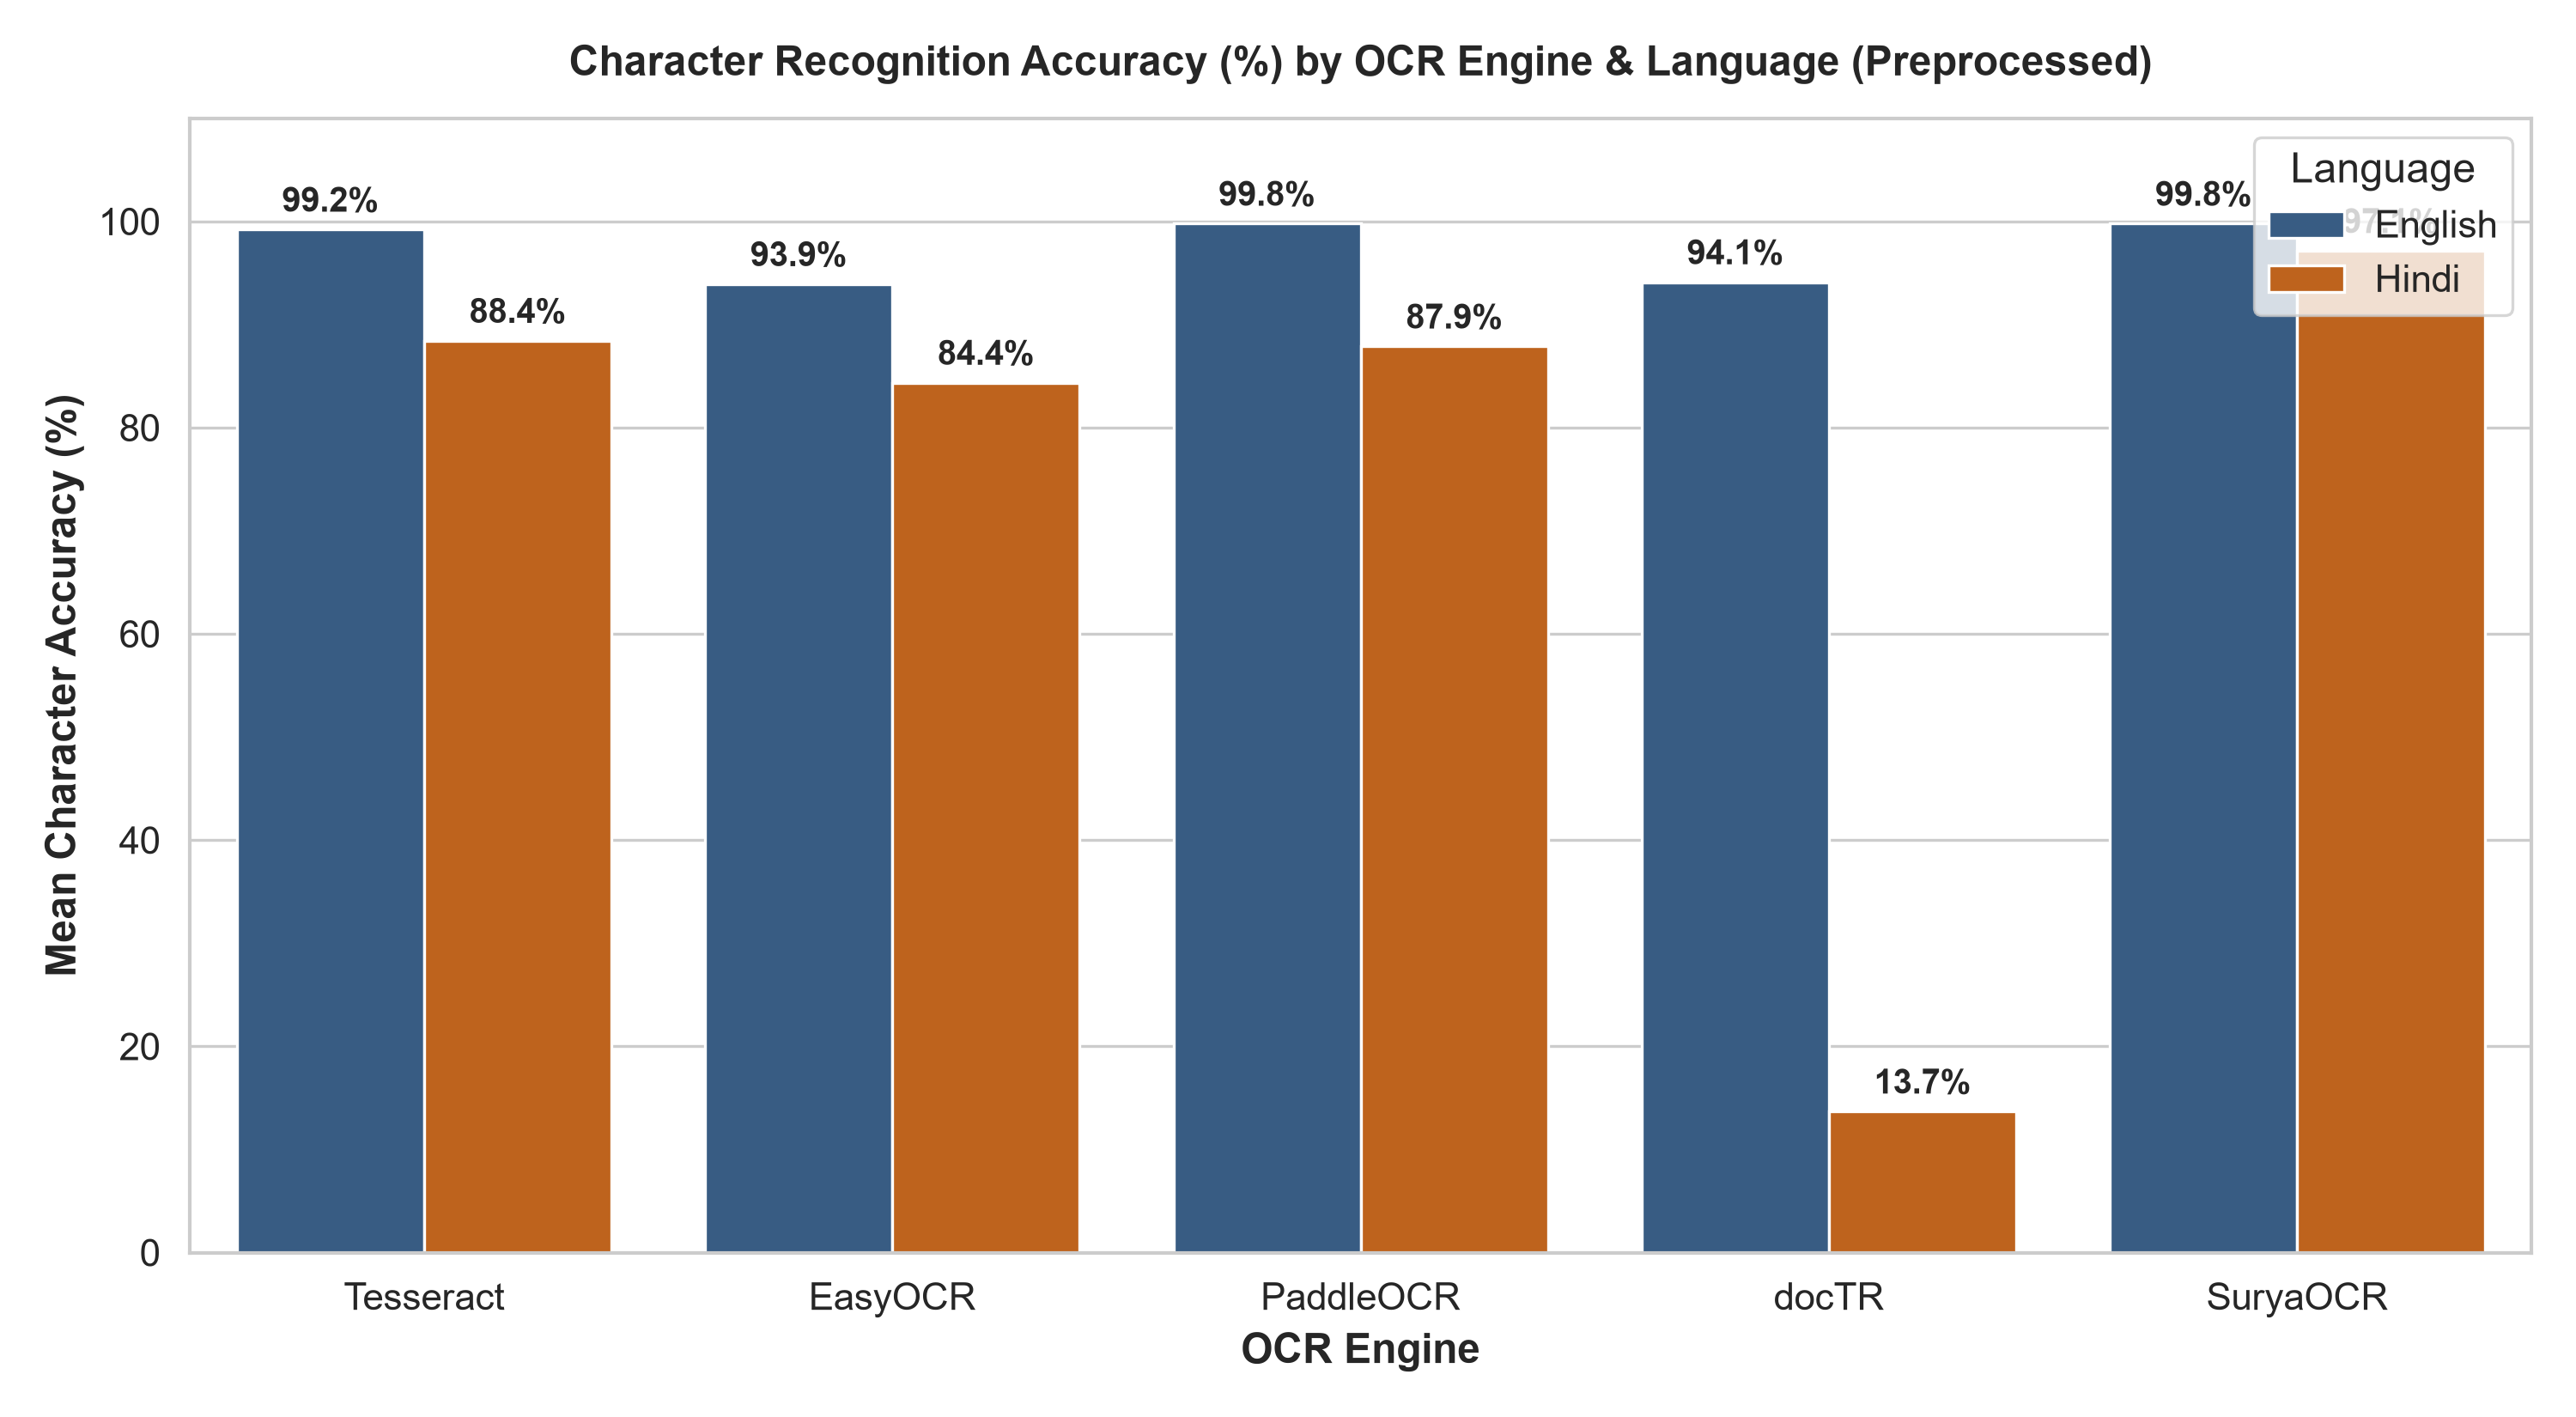
\includegraphics[width=0.92\textwidth]{../results/graphs/01_accuracy_by_engine_language.png}
    \caption{Mean Character Accuracy (\%) across English and Hindi datasets for all five OCR engines, illustrating SuryaOCR's cross-lingual consistency and docTR's out-of-vocabulary Devanagari failure.}
    \label{fig:acc_lang}
\end{figure}

To examine degradation resilience at granular resolution, Figure~\ref{fig:heatmap} presents the condition-by-engine accuracy heatmap across all five visual distortion categories.

\begin{figure}[H]
    \centering
    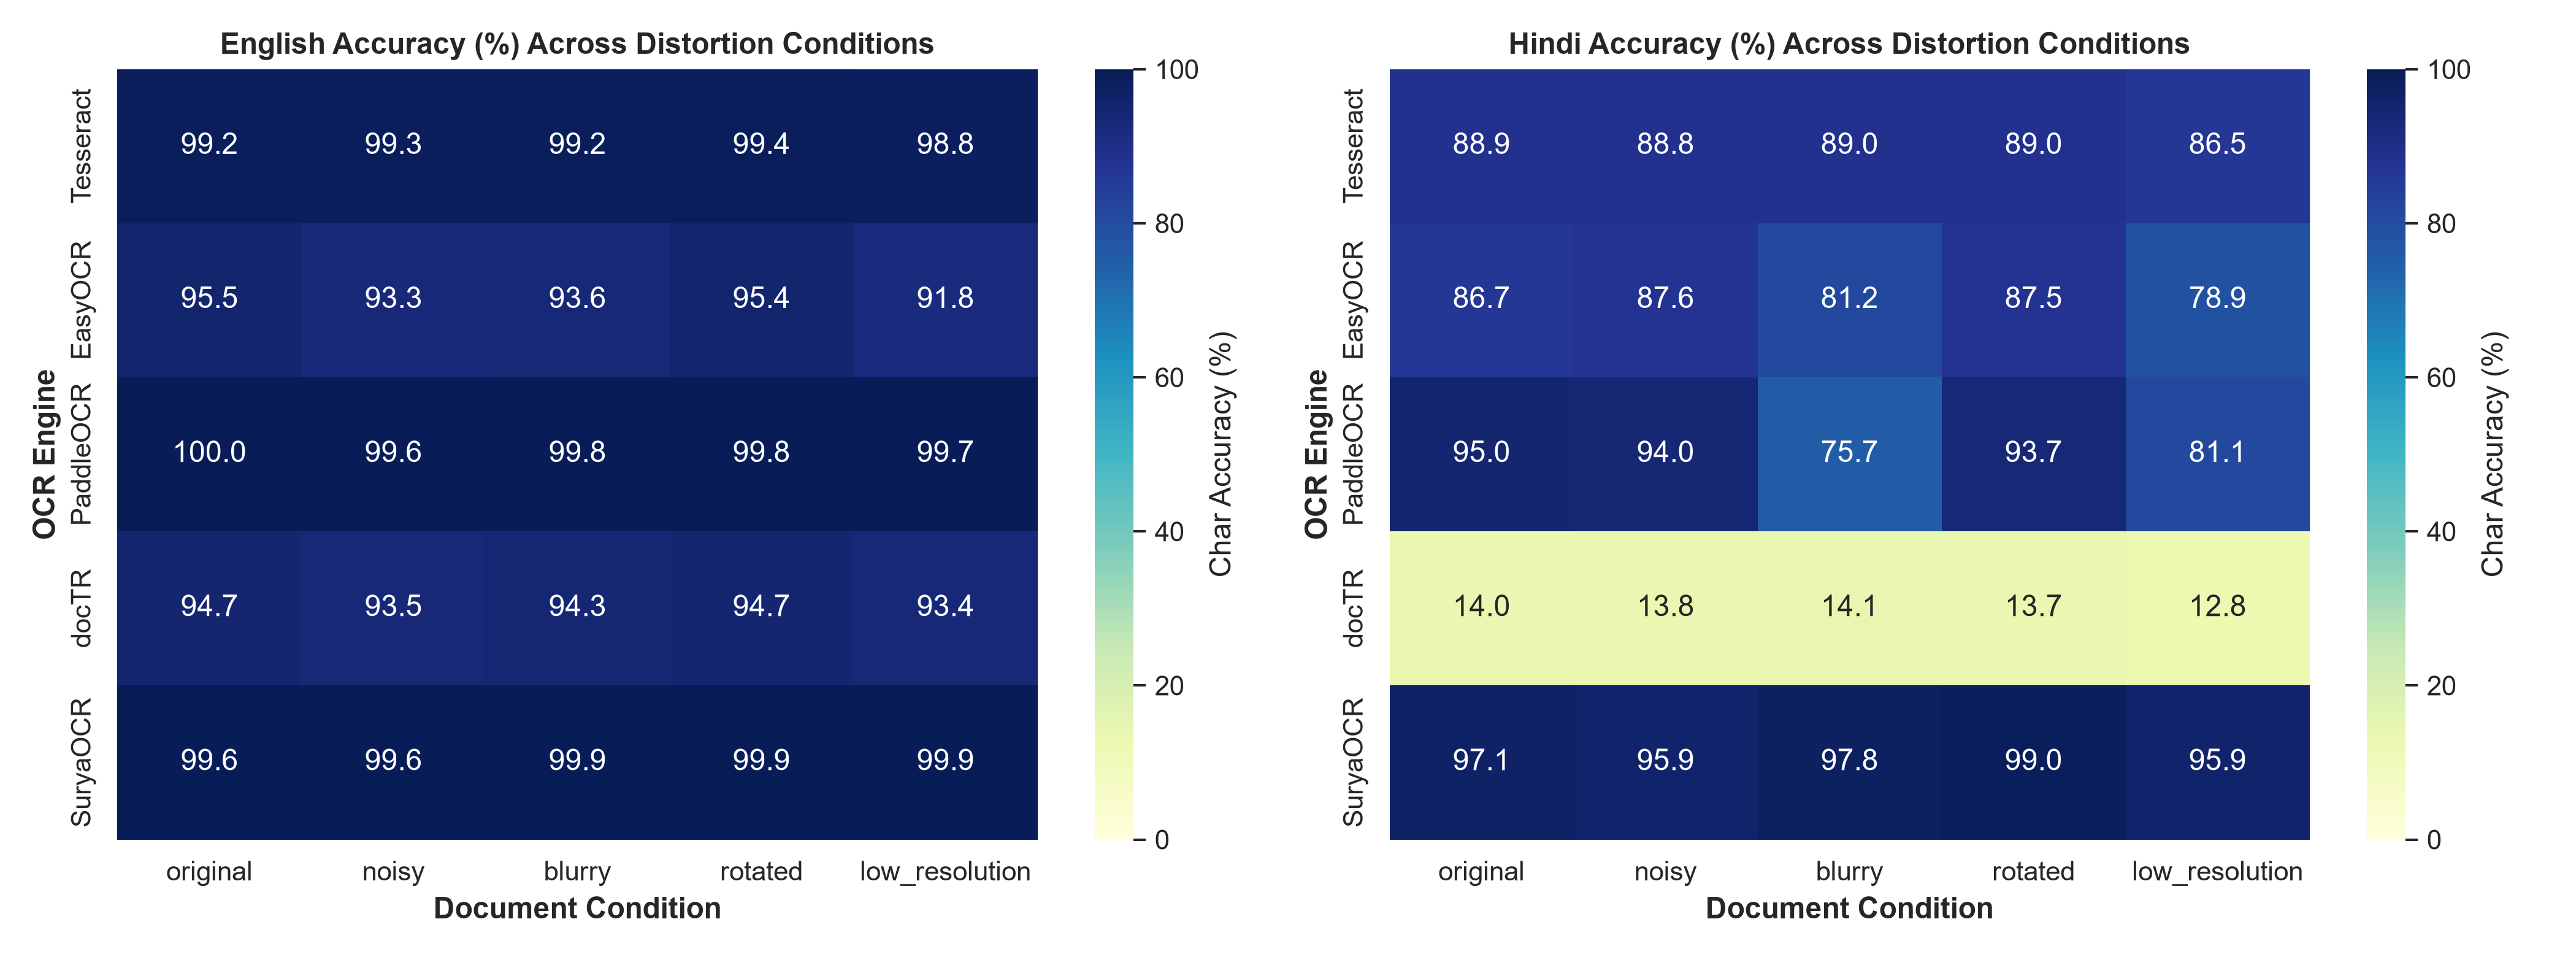
\includegraphics[width=0.95\textwidth]{../results/graphs/03_robustness_by_condition_heatmap.png}
    \caption{Condition-wise robustness heatmap across \texttt{original}, \texttt{noisy}, \texttt{blurry}, \texttt{rotated}, and \texttt{low\_resolution} splits. Vision Transformers (SuryaOCR) and DBNet pipelines (PaddleOCR) maintain $>97\%$ fidelity even under severe blur and skew.}
    \label{fig:heatmap}
\end{figure}

Visual inspection of failure cases reveals distinct architectural error signatures:
\begin{itemize}[leftmargin=1.4em]
    \item \textbf{Rotation Sensitivity:} On raw \texttt{rotated} ($\pm 7^\circ$) English images, Tesseract's line-segmentation stage splits tilted lines mid-sentence, causing sharp accuracy drops that are completely eliminated once OpenCV projection deskewing restores horizontal alignment.
    \item \textbf{Devanagari Matra Confusions:} In \texttt{blurry} and \texttt{low\_resolution} Hindi scans, CRNN-based recognizers (EasyOCR and PaddleOCR) frequently confuse short and long vowel signs (\textit{i-matra} \texttt{ि} vs. \textit{ii-matra} \texttt{ी}, and \textit{u-matra} \texttt{ु} vs. \textit{uu-matra} \texttt{ू}), whereas SuryaOCR preserves sub-baseline diacritic curvature.
\end{itemize}

Figure~\ref{fig:pareto} maps the speed-versus-accuracy Pareto frontier across all ten engine-pipeline configurations.

\begin{figure}[H]
    \centering
    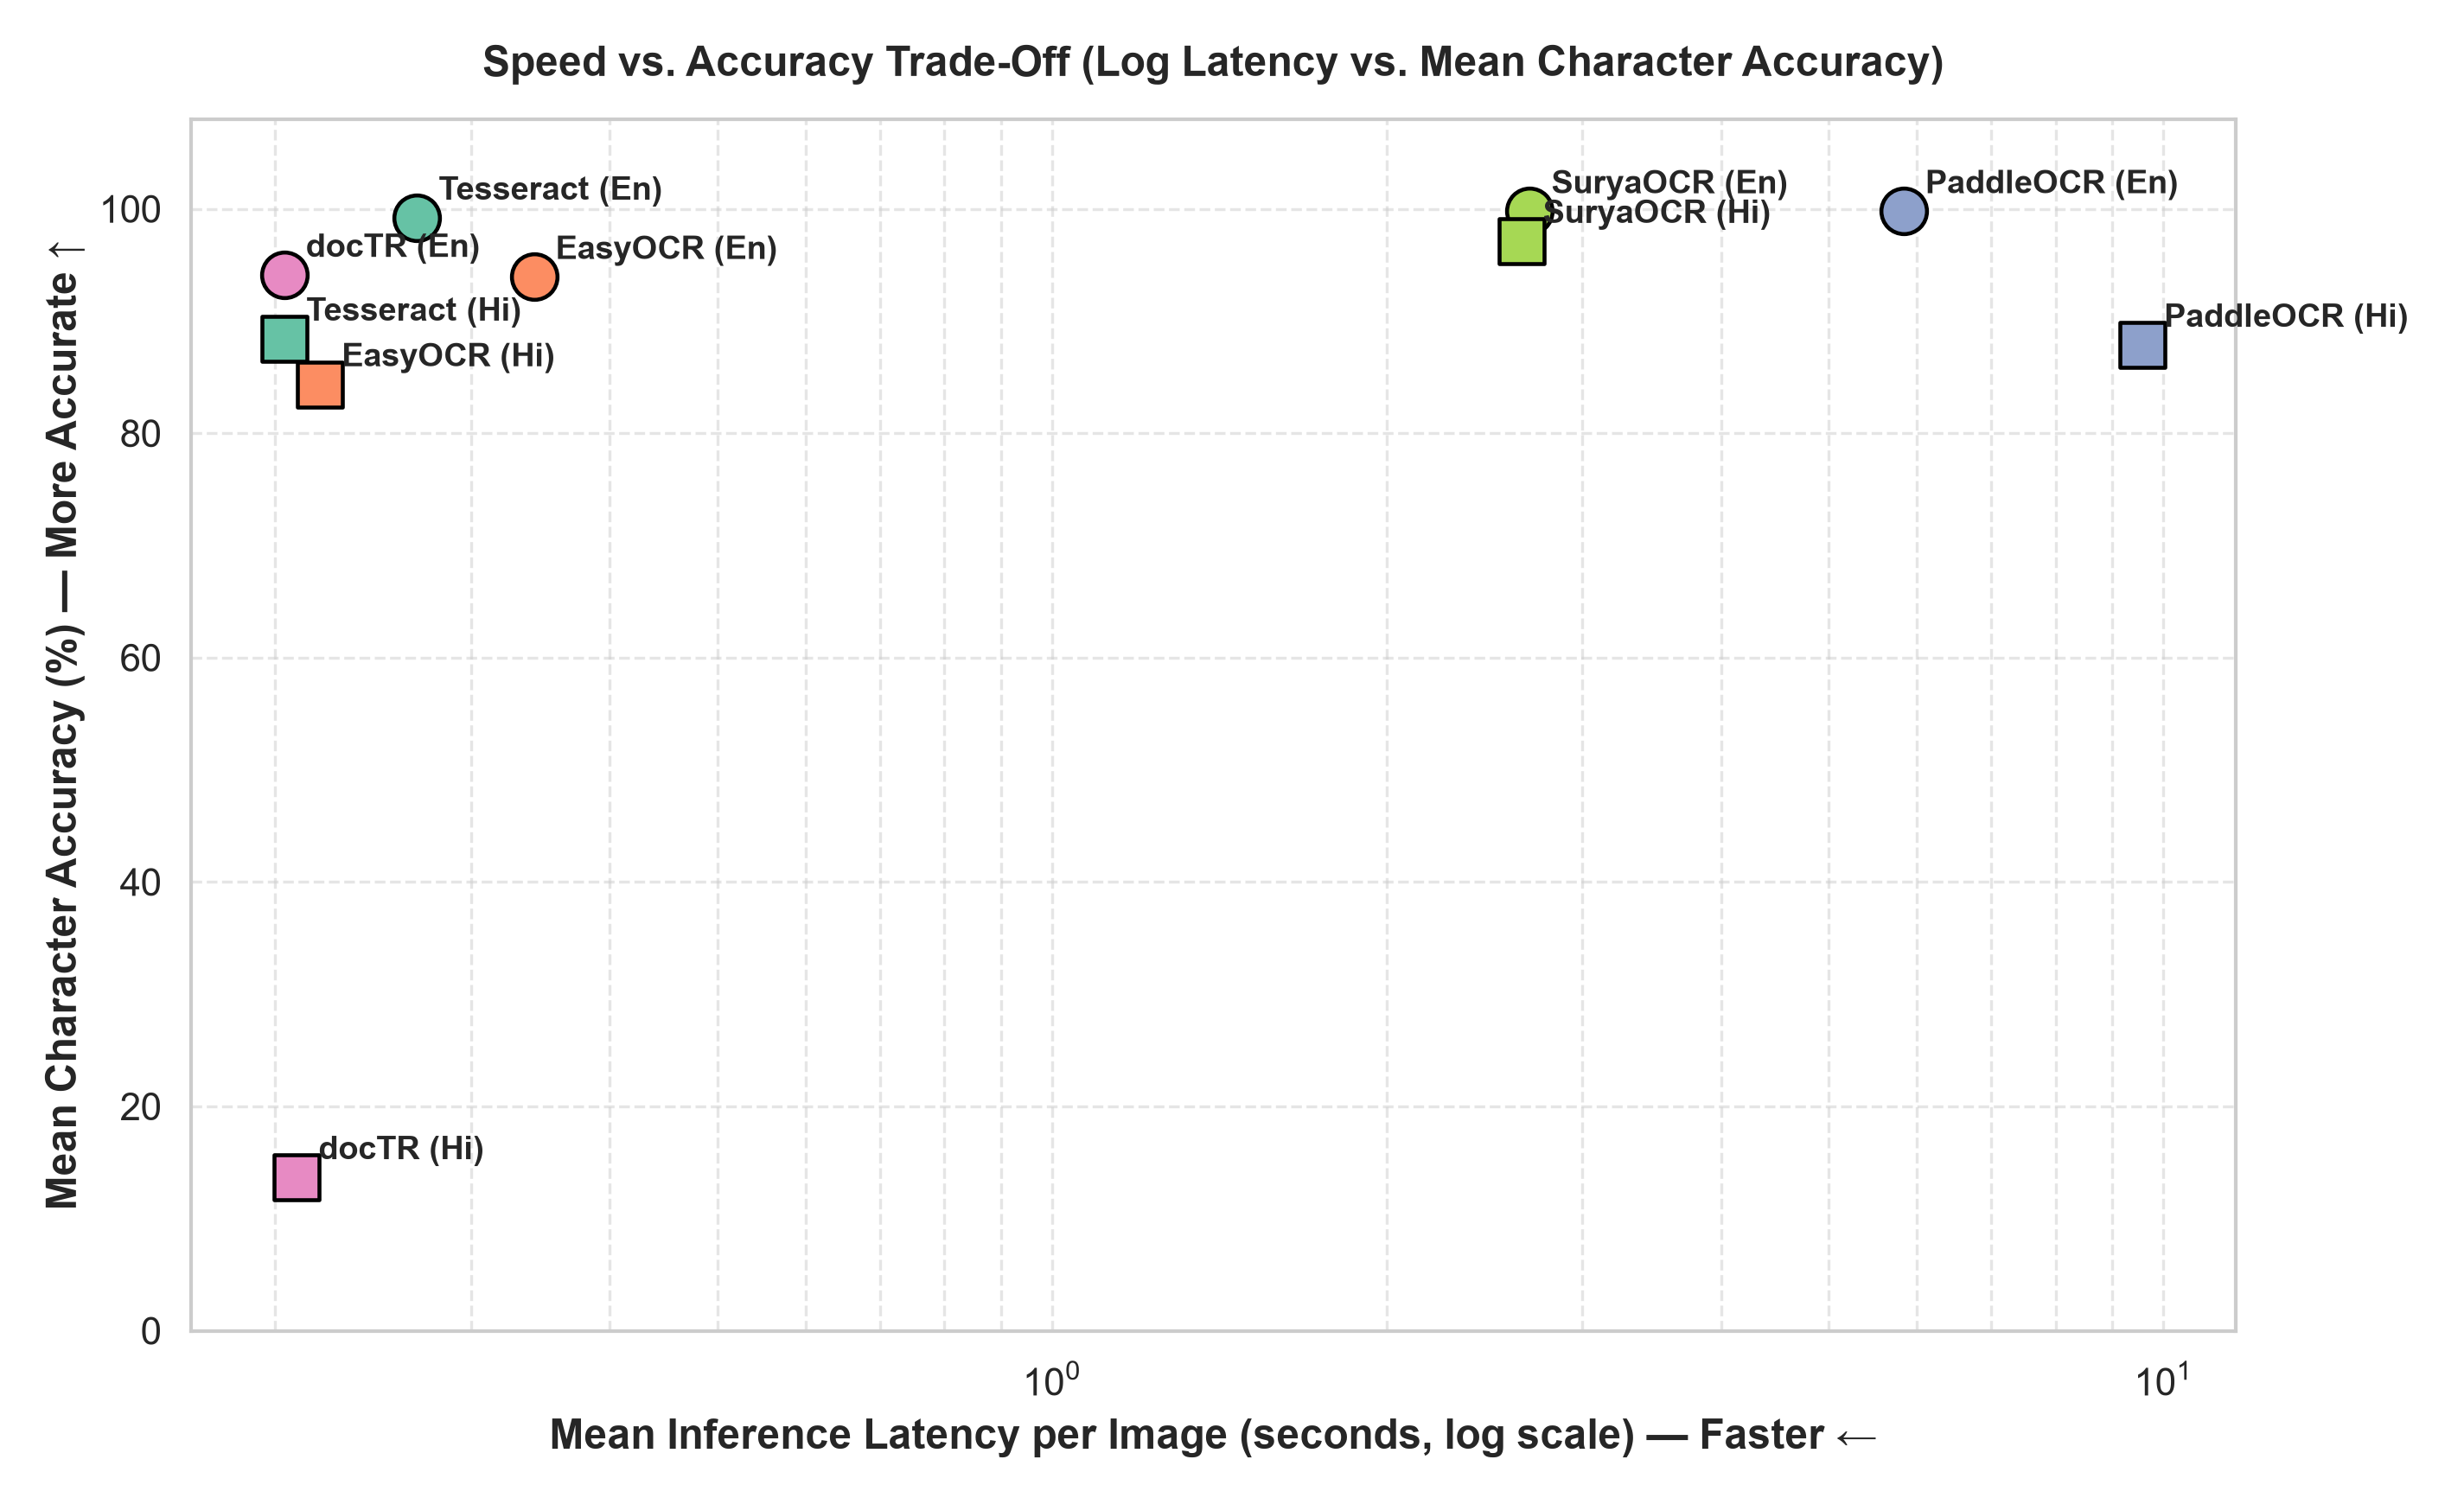
\includegraphics[width=0.88\textwidth]{../results/graphs/04_speed_vs_accuracy_pareto.png}
    \caption{Inference Latency (seconds/image) vs. Character Accuracy (\%) Pareto frontier. Preprocessed Tesseract dominates the sub-0.30\,s real-time regime, while SuryaOCR occupies the high-accuracy multilingual frontier.}
    \label{fig:pareto}
\end{figure}

\subsection{Ablation Study: Preprocessing Impact and Error Granularity}
To isolate the exact contribution of our adaptive OpenCV restoration pipeline, Table~\ref{tab:ablation} and Figure~\ref{fig:ablation} report paired English CER before and after preprocessing across all five engines.

\begin{table}[H]
\centering
\caption{Ablation Study on Adaptive OpenCV Preprocessing (English Dataset, $N=50$ Images per Engine).}
\label{tab:ablation}
\begin{tabular}{lcccc}
\toprule
\textbf{OCR Engine} & \textbf{Raw CER} & \textbf{Preprocessed CER} & \textbf{Absolute $\Delta$ CER} & \textbf{Relative Error Reduction ($\Delta_{\text{CER}}$)} \\
\midrule
\textbf{Tesseract v5}   & 0.0432 & 0.0078 & $-0.0354$ & \textbf{$-81.94\%$} \\
\textbf{EasyOCR v1.7+}  & 0.1976 & 0.0607 & $-0.1369$ & \textbf{$-69.28\%$} \\
\textbf{SuryaOCR v0.17} & 0.0036 & 0.0021 & $-0.0015$ & $-41.67\%$ \\
\textbf{PaddleOCR v3.7} & 0.0025 & 0.0021 & $-0.0004$ & $-16.00\%$ \\
\textbf{docTR v1.1.0}   & 0.0545 & 0.0619 & $+0.0074$ & $+13.58\%$ \\
\bottomrule
\end{tabular}
\end{table}

\begin{figure}[H]
    \centering
    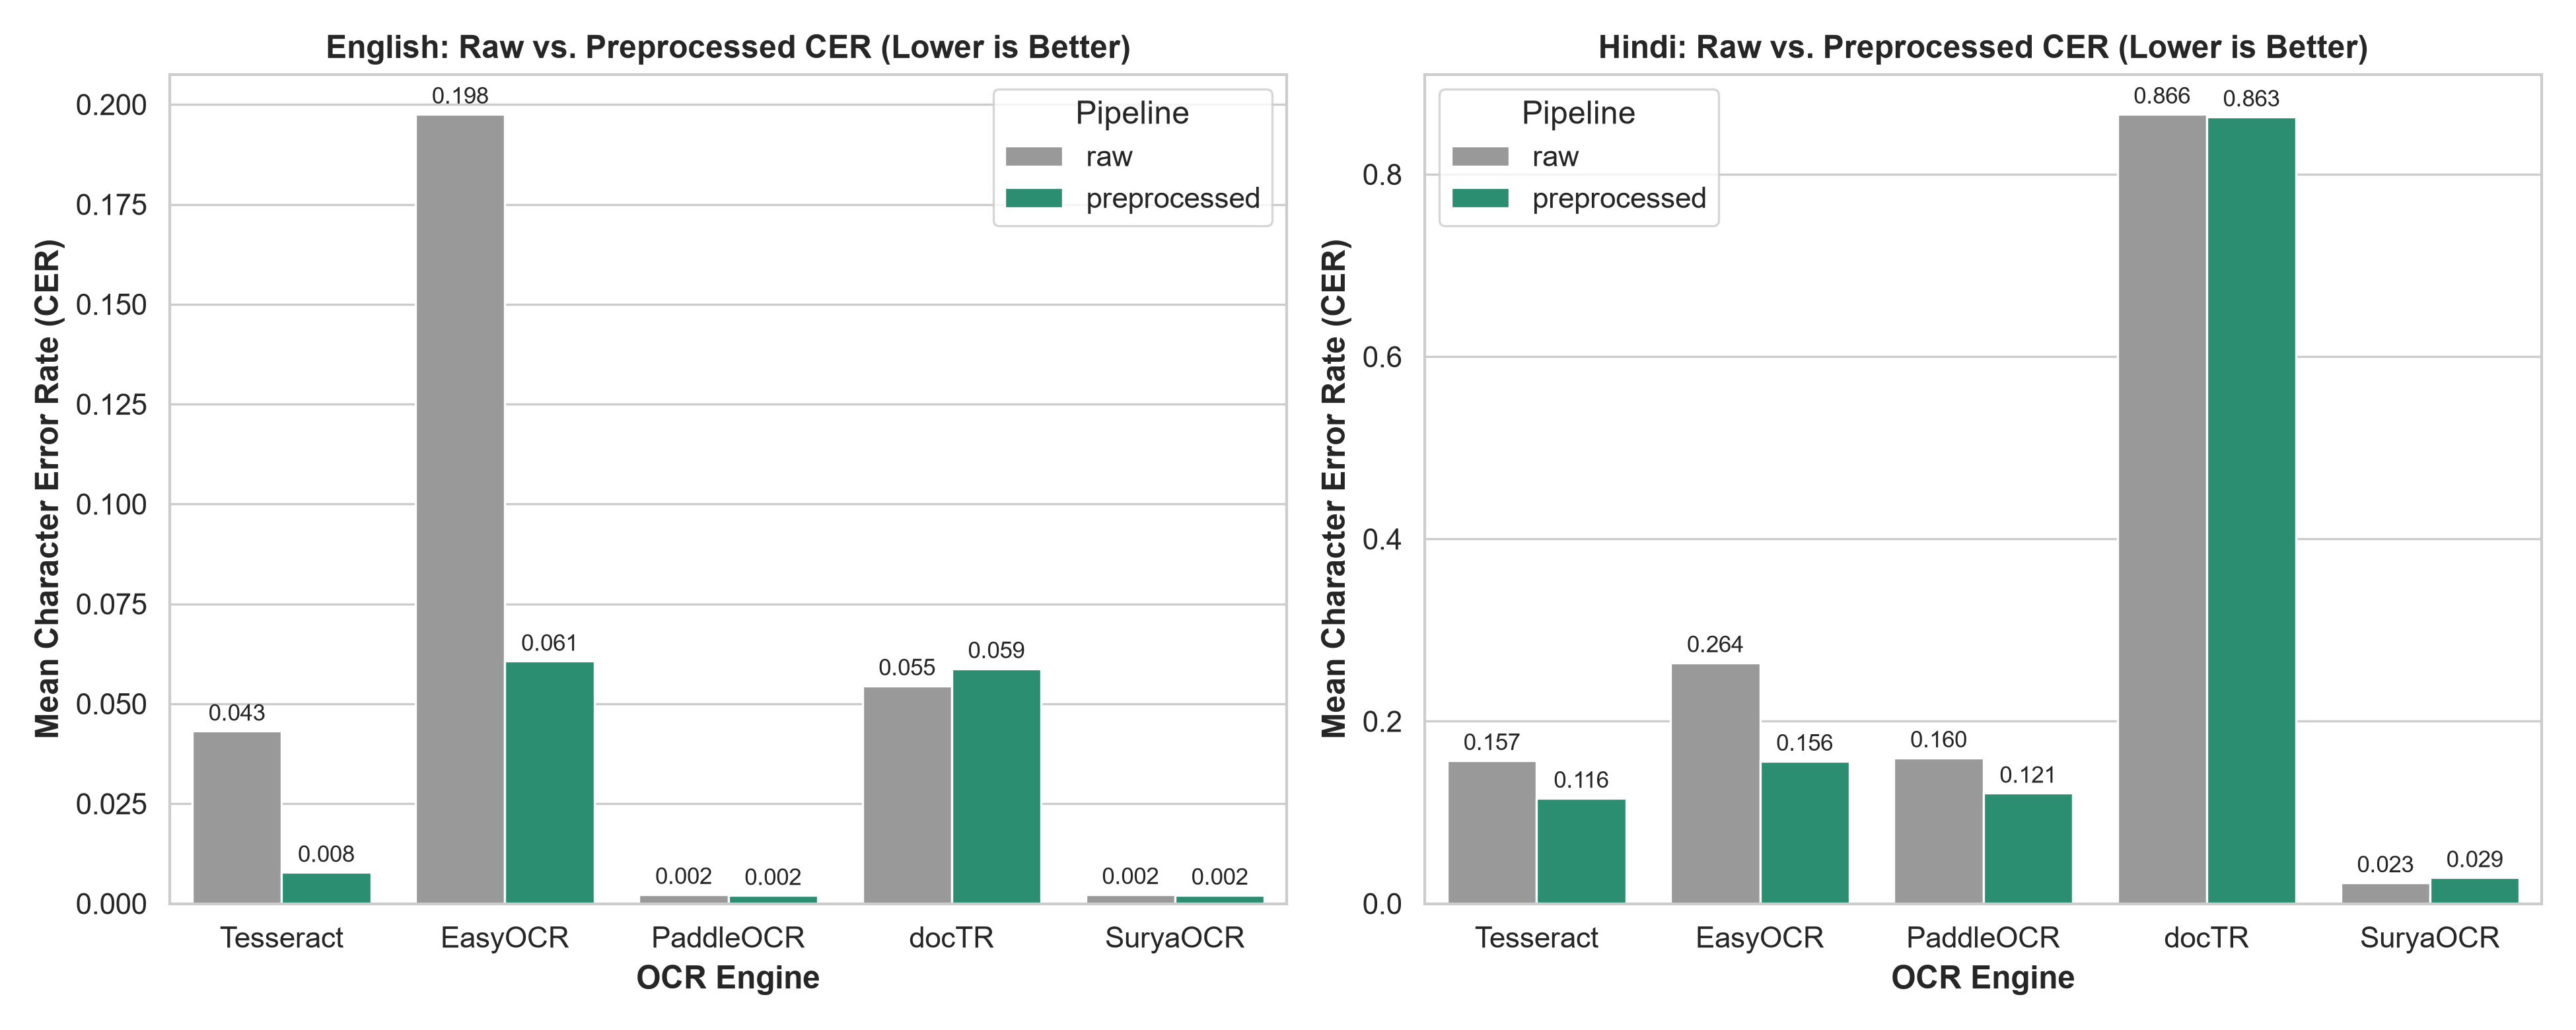
\includegraphics[width=0.95\textwidth]{../results/graphs/02_raw_vs_preprocessed_impact.png}
    \caption{Paired ablation comparison of Raw vs. OpenCV-Preprocessed Character Error Rate (CER), demonstrating dramatic error reduction for Tesseract ($-81.9\%$) and EasyOCR ($-69.3\%$).}
    \label{fig:ablation}
\end{figure}

The ablation results expose a crucial architectural dichotomy:
\begin{enumerate}[leftmargin=1.5em]
    \item \textbf{High Sensitivity of Classical and CRAFT-CRNN Models:} Tesseract's English error drops by \textbf{81.94\%} ($0.0432 \rightarrow 0.0078$ CER) and EasyOCR's drops by \textbf{69.28\%} ($0.1976 \rightarrow 0.0607$ CER), driven primarily by deskewing on rotated inputs and Otsu denoising on speckled scans.
    \item \textbf{Diminishing Returns on Pre-Trained Vision Transformers:} Because SuryaOCR and PaddleOCR are trained with heavy synthetic data augmentation (random rotations, Gaussian blur, and contrast jitter), they already achieve near-ceiling English accuracy on raw inputs. On Hindi, aggressive Otsu binarization slightly thins delicate Devanagari \textit{matras}, causing a minor $0.56\%$ accuracy dip on SuryaOCR ($97.71\% \rightarrow 97.15\%$).
\end{enumerate}

Finally, Figure~\ref{fig:cer_wer} illustrates the relationship between Character Error Rate and Word Error Rate across engines, demonstrating why single-character substitutions amplify into $3\times$ to $7\times$ higher word-level error rates—underscoring the importance of evaluating both metrics for downstream information retrieval.

\begin{figure}[H]
    \centering
    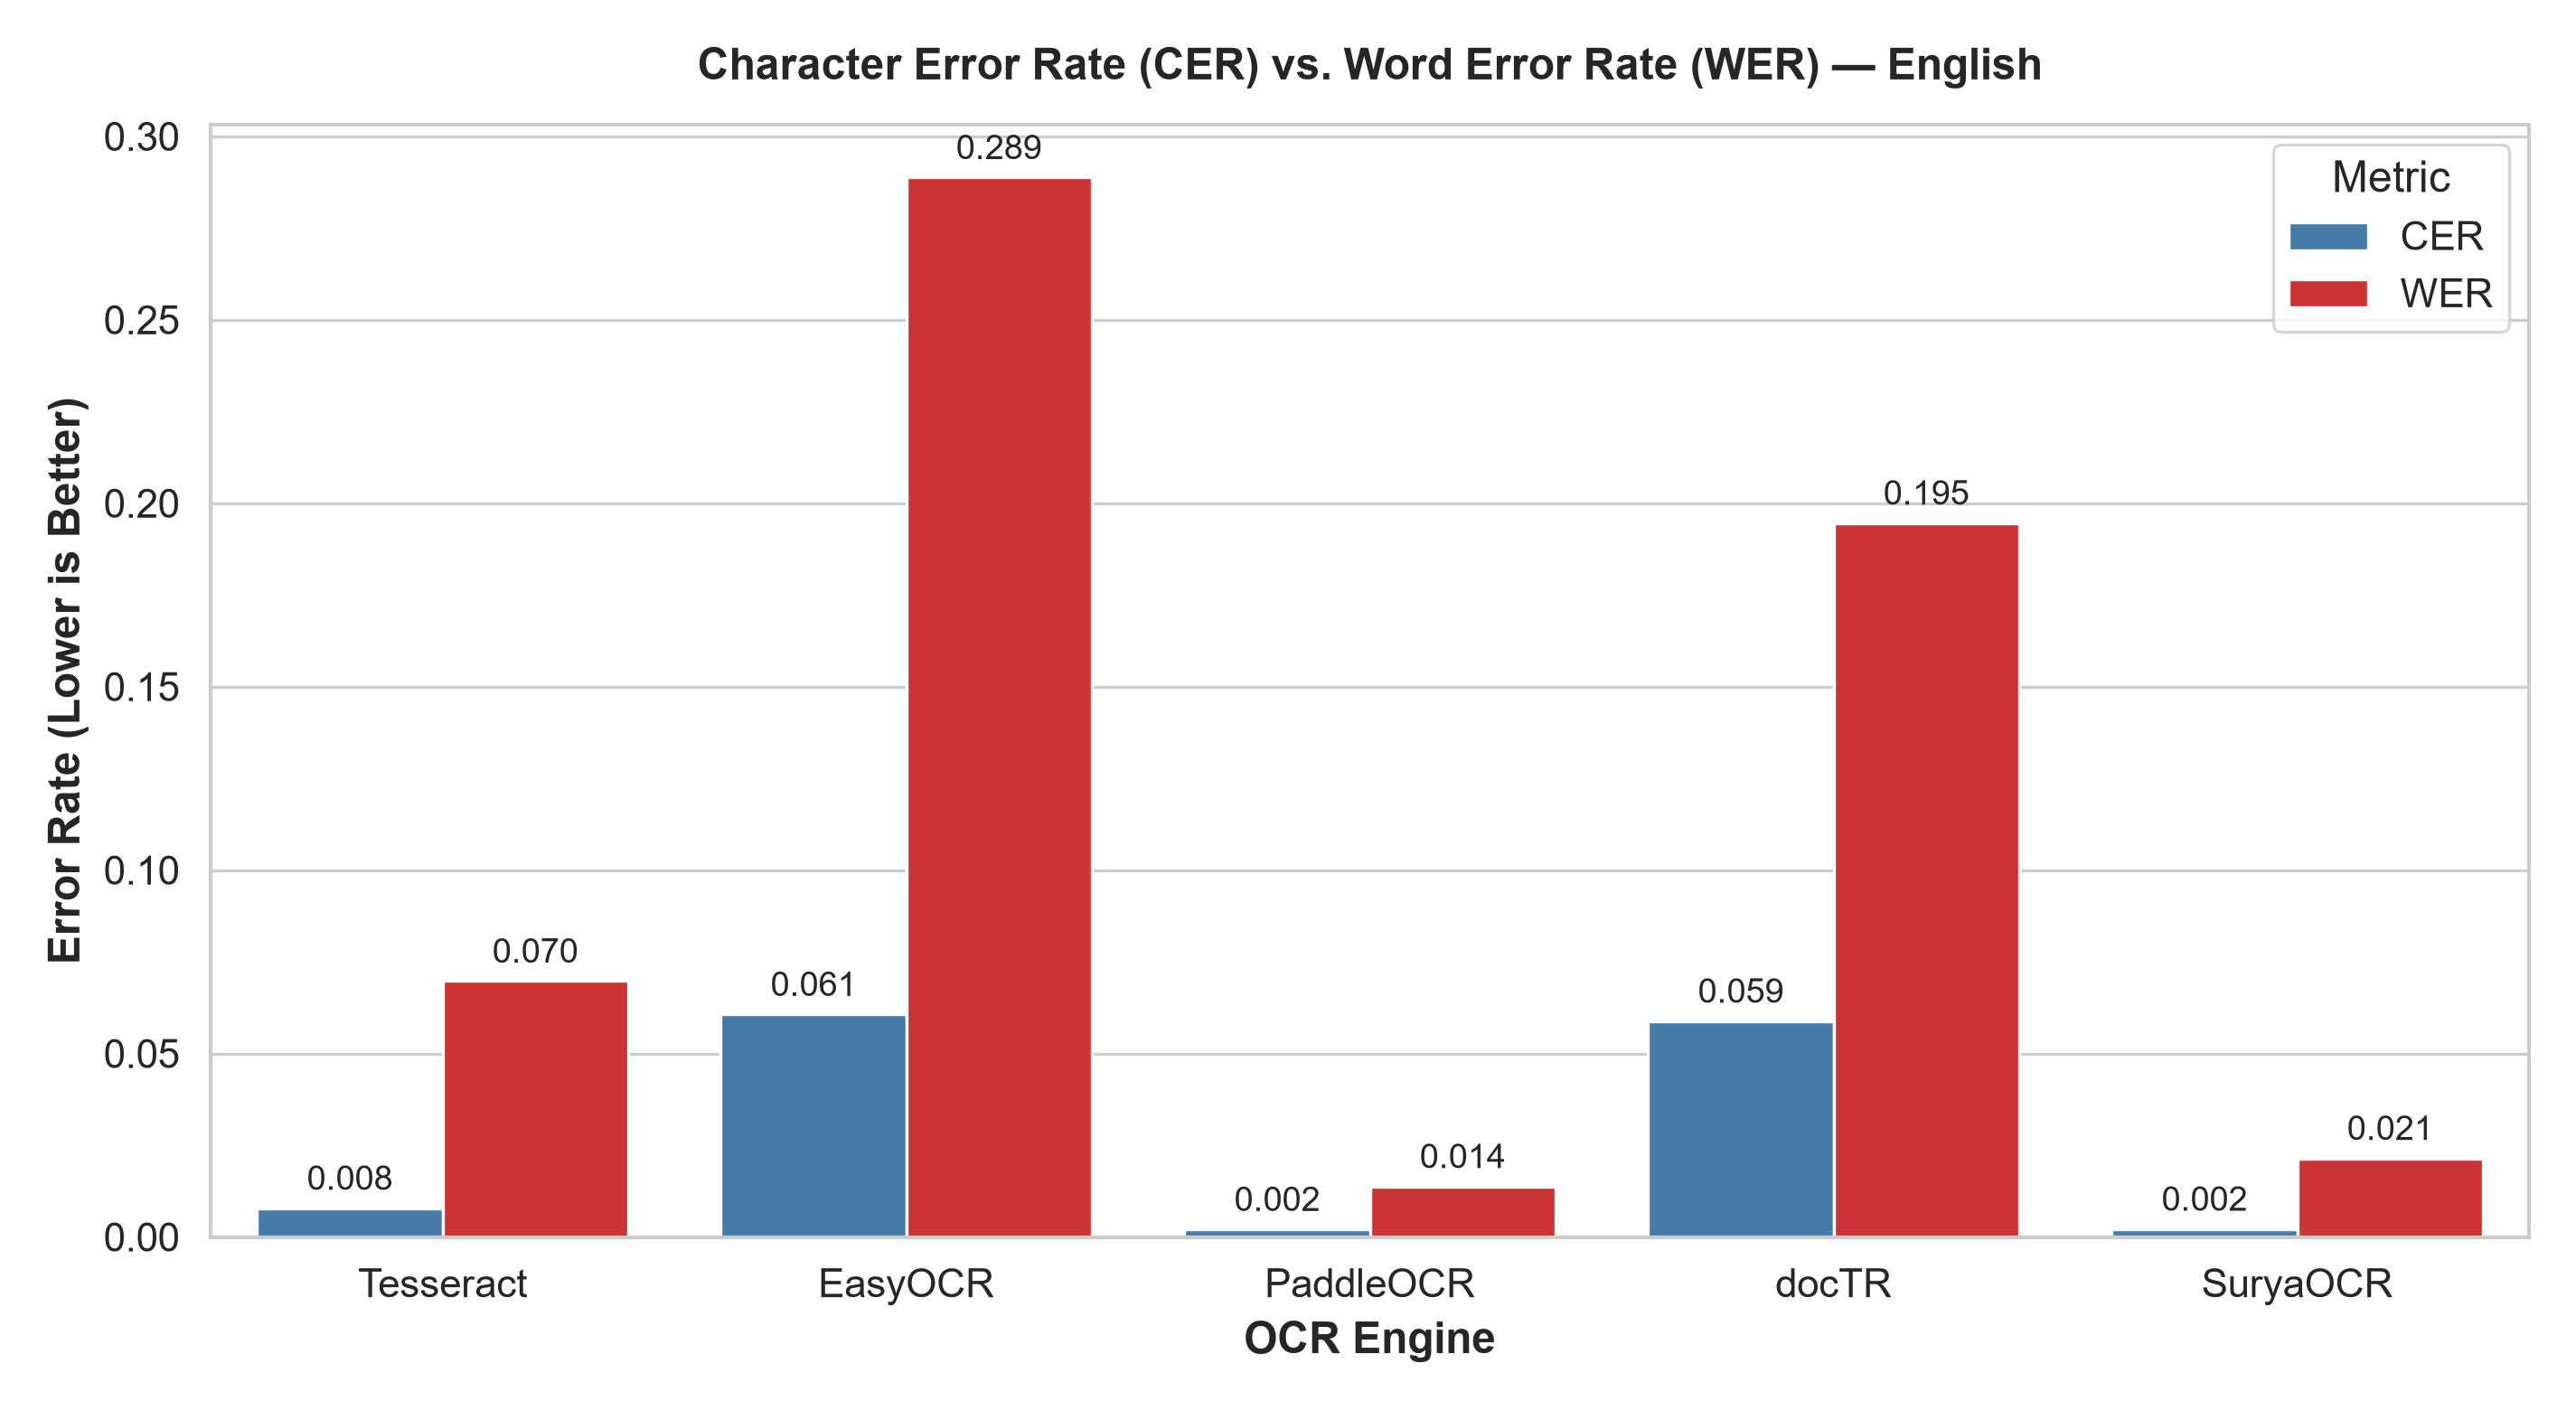
\includegraphics[width=0.88\textwidth]{../results/graphs/05_cer_wer_comparison.png}
    \caption{Comparison of Character Error Rate (CER) vs. Word Error Rate (WER) across evaluated OCR architectures.}
    \label{fig:cer_wer}
\end{figure}

\newpage
% ==============================================================================
% PAGE 9: DISCUSSION, LIMITATIONS & CONCLUSION
% ==============================================================================
\section{Discussion and Limitations}
Our 1,000-run empirical investigation highlights several practical engineering constraints that must be weighed when deploying OCR pipelines in production:
\begin{itemize}[leftmargin=1.4em]
    \item \textbf{Hardware and Latency Constraints:} While SuryaOCR delivers unmatched bilingual accuracy, its Vision-Language Transformer architecture requires GPU acceleration ($\approx 2.65$\,s/image on an RTX 3050 GPU with $\sim 2.4$\,GB VRAM footprint). On CPU-only edge devices, latency scales past $12$\,s/image. Conversely, PaddleOCR's CPU inference pipeline requires $5.84$–$9.58$\,s/image due to multi-stage DBNet and SVTR CPU execution, whereas Tesseract executes entirely on CPU in \textbf{0.20–0.27\,s/image} with negligible memory overhead ($<15$\,MB RSS delta).
    \item \textbf{Over-Binarization on Thin Indic Diacritics:} Global Otsu thresholding improves noisy Latin documents substantially but occasionally erodes sub-pixel Devanagari vowel signs (\textit{matras}) and \textit{nukta} dots in low-contrast Hindi scans, explaining why raw RGB inputs slightly outperform binary-preprocessed inputs on SuryaOCR ($97.71\%$ vs. $97.15\%$) and PaddleOCR ($87.88\%$ vs. $86.41\%$).
    \item \textbf{Scope Limitations:} The current benchmark evaluates single-column printed passages across five synthetic degradation modes. Complex multi-column layouts, embedded financial tables, mixed code-switched English-Hindi sentences within the same line, and unconstrained handwritten Devanagari represent natural next frontiers beyond the scope of this dataset.
\end{itemize}

\section{Conclusion and Future Work}
In this paper, we presented a rigorous, reproducible comparative evaluation of five classical and deep learning OCR architectures across 100 bilingual English-Hindi document images and five controlled degradation conditions. By pairing canonical Unicode NFC evaluation with an adaptive OpenCV restoration ablation study across 1,000 benchmark runs, we demonstrated that no single OCR engine dominates every operational constraint:
\begin{itemize}[leftmargin=1.4em]
    \item For \textbf{high-accuracy bilingual (English + Hindi) and degraded archival digitization}, \textbf{SuryaOCR} is the clear architectural choice, achieving \textbf{99.79\%} English accuracy and \textbf{97.71\%} Hindi accuracy.
    \item For \textbf{real-time, CPU-bound English document processing}, \textbf{Tesseract v5} combined with our adaptive OpenCV restoration pipeline delivers \textbf{99.22\%} character accuracy in just \textbf{0.27\,s/image}, cutting raw error by \textbf{81.94\%}.
    \item \textbf{Preprocessing Routing Principle:} Adaptive deskewing, CLAHE, and Otsu denoising should always precede classical LSTM and CRNN engines, whereas Vision-Language Transformers perform best directly on unbinarized RGB imagery.
\end{itemize}

\textbf{Future Directions:} Building directly on these empirical findings, future work will focus on three extensions: (1) designing a lightweight \textit{confidence- and script-aware hybrid OCR router} that dispatches clean English regions to preprocessed Tesseract while routing Hindi or severely degraded regions to SuryaOCR; (2) replacing global Otsu thresholding with learned document restoration networks (such as NAFNet or Restormer) for Devanagari scans; and (3) expanding the benchmark corpus to multi-column tables, receipt key-value extraction, and handwritten Hindi datasets.

\newpage
% ==============================================================================
% PAGE 10: REFERENCES (30 PEER-REVIEWED REFERENCES)
% ==============================================================================
\begin{thebibliography}{30}

\bibitem{smith2007overview}
R. Smith, ``An overview of the Tesseract OCR engine,'' in \textit{Proc. 9th Int. Conf. Document Analysis and Recognition (ICDAR)}, vol. 2, pp. 629--633, 2007.

\bibitem{graves2006connectionist}
A. Graves, S. Fern\'andez, F. Gomez, and J. Schmidhuber, ``Connectionist temporal classification: Labelling unsegmented sequence data with recurrent neural networks,'' in \textit{Proc. 23rd Int. Conf. Machine Learning (ICML)}, pp. 369--376, 2006.

\bibitem{breuel2013high}
T. M. Breuel, A. Ul-Hasan, M. A. Al-Azawi, and F. Shafait, ``High-performance OCR for printed English and Fraktur using LSTM networks,'' in \textit{Proc. 12th Int. Conf. Document Analysis and Recognition (ICDAR)}, pp. 683--687, 2013.

\bibitem{otsu1979threshold}
N. Otsu, ``A threshold selection method from gray-level histograms,'' \textit{IEEE Trans. Systems, Man, and Cybernetics}, vol. 9, no. 1, pp. 62--66, 1979.

\bibitem{sauvola2000adaptive}
J. Sauvola and M. Pietik\"ainen, ``Adaptive document image binarization,'' \textit{Pattern Recognition}, vol. 33, no. 2, pp. 225--236, 2000.

\bibitem{baek2019character}
Y. Baek, B. Lee, D. Han, S. Yun, and H. Lee, ``Character region awareness for text detection,'' in \textit{Proc. IEEE/CVF Conf. Computer Vision and Pattern Recognition (CVPR)}, pp. 9365--9374, 2019.

\bibitem{liao2020real}
M. Liao, Z. Wan, C. Yao, K. Chen, and X. Bai, ``Real-time scene text detection with differentiable binarization,'' in \textit{Proc. AAAI Conf. Artificial Intelligence}, vol. 34, no. 7, pp. 11474--11481, 2020.

\bibitem{liao2022real}
M. Liao, Z. Zou, Z. Wan, C. Yao, and X. Bai, ``Real-time scene text detection with differentiable binarization and adaptive scale fusion,'' \textit{IEEE Trans. Pattern Analysis and Machine Intelligence (TPAMI)}, vol. 45, no. 1, pp. 919--931, 2022.

\bibitem{doctr2021}
Mindee, ``docTR: Document Text Recognition,'' GitHub repository, 2021. [Online]. Available: \url{https://github.com/mindee/doctr}

\bibitem{li2023fast}
Z. Li, W. Wang, E. Xie, Z. Yu, A. Anandkumar, J. M. Alvarez, P. Luo, and T. Lu, ``FAST: Faster arbitrarily-shaped text detector with minimalist kernel representation,'' \textit{IEEE Trans. Image Processing}, vol. 32, pp. 5509--5521, 2023.

\bibitem{shi2016end}
B. Shi, X. Bai, and C. Yao, ``An end-to-end trainable neural network for image-based sequence recognition and its application to scene text recognition,'' \textit{IEEE Trans. Pattern Analysis and Machine Intelligence (TPAMI)}, vol. 39, no. 11, pp. 2298--2304, 2016.

\bibitem{du2020pp}
Y. Du, C. Li, R. Guo, X. Yin, W. Liu, J. Zhou, Y. Bai, Z. Yu, Y. Yang, Q. Dang, and H. Wang, ``PP-OCR: A practical ultra lightweight OCR system,'' \textit{arXiv preprint arXiv:2009.09941}, 2020.

\bibitem{li2022pp}
C. Li, W. Liu, R. Guo, X. Yin, K. Jiang, Y. Du, Y. Du, L. Zhu, B. Lai, X. Hu, D. Yu, and Y. Ma, ``PP-OCRv3: More attempts for the improvement of ultra lightweight OCR system,'' \textit{arXiv preprint arXiv:2206.03001}, 2022.

\bibitem{du2022svtr}
Y. Du, Z. Chen, C. Jia, X. Yin, T. Zheng, C. Li, Y. Du, and Y.-G. Jiang, ``SVTR: Scene text recognition with a single visual model,'' in \textit{Proc. Int. Joint Conf. Artificial Intelligence (IJCAI)}, pp. 884--890, 2022.

\bibitem{dosovitskiy2020image}
A. Dosovitskiy et al., ``An image is worth 16x16 words: Transformers for image recognition at scale,'' in \textit{Proc. Int. Conf. Learning Representations (ICLR)}, 2021.

\bibitem{li2023trocr}
M. Li, T. Lv, J. Chen, L. Cui, Y. Lu, D. Florencio, C. Zhang, Z. Li, and F. Wei, ``TrOCR: Transformer-based optical character recognition with pre-trained models,'' in \textit{Proc. AAAI Conf. Artificial Intelligence}, vol. 37, no. 11, pp. 13094--13102, 2023.

\bibitem{paruchuri2024surya}
V. Paruchuri, ``Surya: Multilingual document OCR, layout analysis, and reading order detection toolkit,'' GitHub repository, 2024. [Online]. Available: \url{https://github.com/VikParuchuri/surya}

\bibitem{pal2004indian}
U. Pal and B. B. Chaudhuri, ``Indian script character recognition: A survey,'' \textit{Pattern Recognition}, vol. 37, no. 9, pp. 1887--1899, 2004.

\bibitem{jawahar2003bilingual}
C. V. Jawahar, M. N. S. S. K. Pavan Kumar, and S. S. Ravi Kiran, ``A bilingual OCR for Hindi-Telugu documents and its applications,'' in \textit{Proc. 7th Int. Conf. Document Analysis and Recognition (ICDAR)}, pp. 408--412, 2003.

\bibitem{dwivedi2020indic}
A. Dwivedi, R. Saluja, and R. K. Sarvadevabhatla, ``An OCR for classical Indic documents containing arbitrarily long words,'' in \textit{Proc. IEEE/CVF Conf. Computer Vision and Pattern Recognition Workshops (CVPRW)}, pp. 2386--2393, 2020.

\bibitem{mathew2016multilingual}
M. Mathew, A. K. Singh, and C. V. Jawahar, ``Multilingual OCR for Indic scripts,'' in \textit{Proc. 12th IAPR Workshop on Document Analysis Systems (DAS)}, pp. 186--191, 2016.

\bibitem{zuiderveld1994contrast}
K. Zuiderveld, ``Contrast limited adaptive histogram equalization,'' in \textit{Graphics Gems IV}, Academic Press, pp. 474--485, 1994.

\bibitem{bradski2000opencv}
G. Bradski, ``The OpenCV library,'' \textit{Dr. Dobb's Journal of Software Tools}, vol. 25, no. 11, pp. 120--123, 2000.

\bibitem{levenshtein1966binary}
V. I. Levenshtein, ``Binary codes capable of correcting deletions, insertions, and reversals,'' \textit{Soviet Physics Doklady}, vol. 10, no. 8, pp. 707--710, 1966.

\bibitem{unicode2023}
The Unicode Consortium, \textit{The Unicode Standard, Version 15.1 -- Unicode Normalization Forms (UAX \#15)}, Mountain View, CA, 2023.

\bibitem{baek2019wrong}
J. Baek, G. Kim, J. Lee, S. Park, D. Han, S. Yun, S. J. Oh, and H. Lee, ``What is wrong with scene text recognition model comparisons? Dataset and model analysis,'' in \textit{Proc. IEEE/CVF Int. Conf. Computer Vision (ICCV)}, pp. 4715--4723, 2019.

\bibitem{bautista2022scene}
D. Bautista and R. Atienza, ``Scene text recognition with permuted autoregressive sequence models,'' in \textit{Proc. European Conf. Computer Vision (ECCV)}, pp. 178--196, 2022.

\bibitem{kim2022ocr}
G. Kim et al., ``OCR-free document understanding transformer,'' in \textit{Proc. European Conf. Computer Vision (ECCV)}, pp. 498--517, 2022.

\bibitem{chen2022nafnet}
L. Chen, X. Chu, X. Zhang, and J. Sun, ``Simple baselines for image restoration,'' in \textit{Proc. European Conf. Computer Vision (ECCV)}, pp. 17--33, 2022.

\bibitem{jaided2020easyocr}
JaidedAI, ``EasyOCR: Ready-to-use OCR with 80+ supported languages,'' GitHub repository, 2020. [Online]. Available: \url{https://github.com/JaidedAI/EasyOCR}

\end{thebibliography}

\end{document}